\vspace*{-0.1in}
\section{Example Architecture}
\label{section-architecture}

\begin{table}[t]
\begin{threeparttable}
{\footnotesize
\begin{tabularx}{\textwidth}{clrlXr}

\multicolumn{1}{c}{\textbf{\large{Type}}} &
\multicolumn{1}{c}{\textbf{\large{Name}}} &
\multicolumn{2}{c}{\textbf{\large{Power (mW)}}} &
\multicolumn{1}{c}{\textbf{\large{Performance}}} &
\multicolumn{1}{c}{\textbf{\large{ID}}}
\\ \toprule 

\multirow{6}{*}{\vspace{-0.15in}\textbf{CPU}} &
\multirow{2}{*}{ARM Cortex-M4\tnote{11}~\cite{cortexm4-web}} &
0.9\tnote{1} & &
75 MHz, 94 MIPS\tnote{2} &
\multirow{2}{*}{\textbf{P1}}
\\

& & &
15.6 &
300 MHz, 375 MIPS
&
\\ \cmidrule(l){2-6}

& \multirow{2}{*}{ARM Cortex-R4\tnote{11}~\cite{cortexr4-web}} &
4.6\tnote{1} & &
206 MHz, 342 DMIPS\tnote{2} &
\multirow{2}{*}{\textbf{P2}}
\\

& & &
78.8 &
620 MHz, 1030 DMIPS
&
\\ \cmidrule(l){2-6}

& \multirow{2}{*}{ARM Cortex-A9~\cite{cortexa9-web}} &
23.5\tnote{1} & &
415 MHz, 1037 DMIPS\tnote{2} &
\multirow{2}{*}{\textbf{P3}}
\\

& & &
400 &
830 MHz, 2075 DMIPS
&
\\ \toprule

\multirow{8}{*}{\vspace*{-0.15in}\textbf{Memory}} &
\multirow{2}{*}{\textbf{32~MB} ISSI SDRAM~\cite{issi32MBsdram-datasheet}} &
81 & &
Refresh only &
\multirow{2}{*}{\textbf{M1}}
\\

& & &
108 &
166 MHz
&
\\ \cmidrule(l){2-6}

&
\multirow{2}{*}{\textbf{256~MB} Micron ``Slow'' DDR2} &
239\tnote{10} & &
Refresh only &
\multirow{2}{*}{\textbf{M2}}
\\

& & &
405 &
266 MHz, 478Mtps
&
\\ \cmidrule(l){2-6}

&
\multirow{2}{*}{\textbf{1~GB} Micron ``Slow'' DDR2} &
322\tnote{10} & &
Refresh only &
\multirow{2}{*}{\textbf{M3}}
\\

& & &
482 &
266 MHz, 478Mtps
&
\\ \cmidrule(l){2-6}

%&
%\multirow{2}{*}{\textbf{2~GB} Micron ``Slow'' DDR2} &
%337 & &
%Refresh only &
%\multirow{2}{*}{\textbf{M4}}
%\\
%
%& & &
%582 &
%266 MHz, 478Mtps
%&
%\\ \cmidrule(l){2-6}
%
%&
%\multirow{2}{*}{\textbf{256~MB} Micron ``Fast'' DDR2} &
%346 & &
%Refresh only &
%\multirow{2}{*}{\textbf{M5}}
%\\
%
%& & &
%549 &
%400 Mhz, 720Mtps
%&
%\\ \cmidrule(l){2-6}

&
\multirow{2}{*}{\textbf{1~GB} Micron ``Fast'' DDR2} &
559\tnote{10} & &
Refresh only &
\multirow{2}{*}{\textbf{M4}}
\\

& & &
835 &
400 Mhz, 720Mtps
&
\\ \toprule

\multirow{6}{*}{\vspace*{-0.15in}\textbf{Storage}} &
\multirow{2}{*}{\textbf{2~GB} MicroSD Card} &
20\tnote{5} & &
Idle &
\multirow{2}{*}{\textbf{S1}}
\\

& & &
100\tnote{5} &
25 MBps\tnote{6}
&
\\ \cmidrule(l){2-6}


& \multirow{2}{*}{\textbf{64~GB} OCZ SSD} &
200\tnote{7} & &
Idle &
\multirow{2}{*}{\textbf{S2}}
\\

& & &
1000\tnote{7} &
5.5 MBps\tnote{7}
&
\\ \cmidrule(l){2-6}

& \multirow{2}{*}{\textbf{320~GB} Seagate HDD} &
700\tnote{7} & &
Idle &
\multirow{2}{*}{\textbf{S3}}
\\

& & &
1800\tnote{7} &
1.6 MBps\tnote{7}
&
\\ \toprule

\multirow{6}{*}{\vspace{-0.15in}\textbf{Radio}} &
\multirow{2}{*}{\textbf{250~kbps}} TI CC2540 BLE & 
6.63\tnote{2} & &
10\% duty cycle\tnote{9} &
\multirow{2}{*}{\textbf{R1}}
\\

& & &
66.3\tnote{3} &
Receive mode\tnote{3}
& \\ \cmidrule(l){2-6}

&
\multirow{2}{*}{\textbf{179.2~kbps} EDGE 3G} &
10\tnote{8} & &
Idle &
\multirow{2}{*}{\textbf{R2}}
\\

& & &
1320\tnote{8} &
Transmit mode
& \\ \cmidrule(l){2-6}

&
\multirow{2}{*}{\textbf{11~Mbps} Marvell 88W8686 802.11bg} &
30.9\tnote{2} & &
10\% duty cycle\tnote{9} &
\multirow{2}{*}{\textbf{R3}}
\\

& & &
309.3\tnote{4} &
Idle mode\tnote{4}
& \\ \toprule

\end{tabularx}
}
{\footnotesize
\begin{tablenotes}
\item [1] Optimistic estimate based on an optimistic estimate of DVFS providing 1:5 performance and
1:17 power scaling\cite{jssc02-PowerPC-SoC}.
\item [2] Estimated based on scaled full-power performance.
\item [3] Receive-only in high-sensitivity mode. Transmit numbers are not
significantly higher.
\item [4] Transmit and receive modes have very different power
consumption so usage is workload-dependent.
\item [5] Estimated due to lack of publicly-available datasheets.
\item [6] Maximum achievable.
\item [7] Measured by Tom's Hardware~\cite{ssd-tomshardware} using a realistic read-write mixture workload.
\item [8] Estimated numbers based on 2008
whitepaper~\cite{option3gpower-whitepaper}.
\item [9] Duty cycling allows the receiver to save power by shifting energy
consumption to the sender, which has to remain online (as in 802.11
PSM) or send longer packets (as in 802.15.4 Low-Power
Listening~\cite{tinyos-lpl}).
\item [10] Estimated based on Micron leakage numbers.
\item [11] Capable of running a subset of the full instruction set architecture
used by P3.
\end{tablenotes}
}
\caption{\textbf{Performance and power consumption of various hardware
components.} We assume voltage gating can reduce the power draw of a disabled
component to near zero~\cite{islped-vdd-gate}.}
\end{threeparttable}
\label{table-components}
\end{table}


To begin, we assemble a heterogeneous power-proportional device combining two
general-purpose processors\footnote{Distinguished from task-specific
processors like GPUs or DSPs.}, two memory chips, two storage devices and two
radios. Table~\ref{table-components} presents the components we selected.

The relationship between power and performance varies for each component.
Processors may transition smoothly over a restricted power envelope using
DVFS, but cannot scale to zero due to leakage current. DRAM memory chips have
a constant refresh cost scaling roughly with capacity plus additional power
draw corresponding to the rate of reads and writes. Storage devices differ
based on whether or not they include spinning components. Flash drives do not
and scale approximately with usage but are limited in size. Radios exhibit
wide power-performance variation because their usage depends both on the
hardware and the protocol. 802.11 clients can enter power-saving mode (PSM)
which uses base station buffering to save power. Bluetooth has limited range
but lower power consumption balanced between both sides of the link.

We define a \textit{component ensemble} as the set of components currently
active, constraining the set of valid ensembles to include only those that
can support the device operating system. For our example, these include (a)
one or both processors, (b) one or both memory chips\footnote{While many
low-power processors come with small amounts of integrated memory, we have
conservatively chosen to require 32~MB of RAM in order to run embedded
versions of Linux. It is conceivable that our candidate device could enter an
active sleep state with a micro-kernel capable of fitting in the processor's
onboard RAM.}, (c) zero, one or both storage devices and (d) zero, one or
both radios. By switching between components our device can operate across a
wide power range. It its lowest-power ensemble, the device has a 75~MHz CPU,
32~MB of RAM, and draws 82\footnote{Actual power consumption would be higher
due to system buses, memory controllers, and other components of a complete
architecture.}~mW and is roughly-equivalent to a embedded sensor node. In its
highest-power ensemble the device has multiple cores, over 1~GB of RAM, over
320~GB of storage, Wifi and Bluetooth. Consuming almost 2.5~W, it is similar
to emerging smartphones.

\begin{figure*}[t]
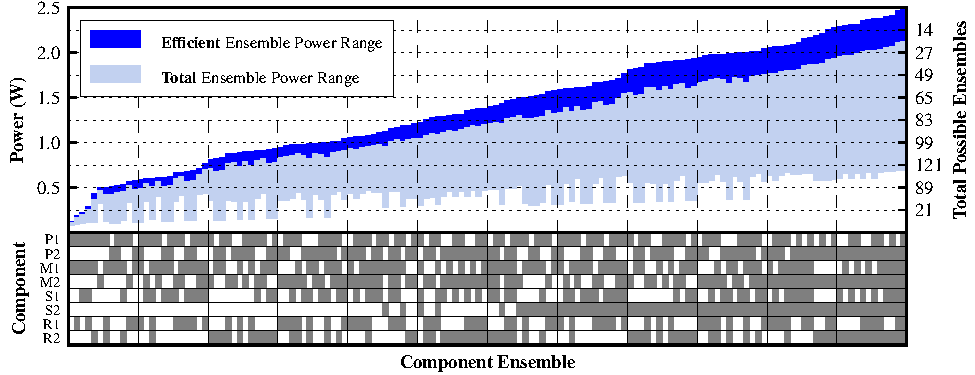
\includegraphics{./figures/componentgraph.pdf}

\caption{\small \textbf{Power envelopes of all 144 example device component
ensembles.} Ensembles are sorted by increasing maximum power draw. For each
ensemble, the bottom shows which components are active and the top displays
the power envelope. The top 80\% of the envelope---the most efficient
operating range---is drawn in dark blue. The right axis counts the total
number of ensembles that might draw that much power: e.g., there are 121
ensembles that could consume 0.75~W, depending on the workload.}

\vspace{0.10in}
\hrule
\vspace{-0.20in}
\label{figure-componentgraph}
\end{figure*}


This device can activate \textit{144 valid component ensembles}\footnote{3
processor choices $\times$ 3 memory choices $\times$ 4 storage choices
$\times$ 4 radio choices.}. Figure~\ref{figure-componentgraph} shows the
composition and power envelope of each, and motivates two observations.
First, there are many valid ensembles and wide usage variation even in an
architecture with only two components per class. Incorporating more
components would produce even more options. Second, at any power level there
are many diverse ensembles the device can use: a fast processor, small memory
chip, and slow disk; a slow processor, large memory chip, and fast radio;
etc. These differ not in their total power consumption but in how they
perform and distribute power across components, and while some ensembles may
seem too weird to be useful they may suit certain applications. Finally,
while it may seem best to avoid inefficient ensembles---those achieving low
utilization and a low active- to idle-power ratio---given the speed of
temporal changes in demand and the overhead of ensemble transitions we expect
devices to spend some time at the low end of ensemble power envelopes.
